% document formatting
\documentclass[10pt]{article}
\usepackage[utf8]{inputenc}
\usepackage[left=1in,right=1in,top=1in,bottom=1in]{geometry}
\usepackage[T1]{fontenc}
\usepackage{xcolor}

% math symbols, etc.
\usepackage{amsmath, amsfonts, amssymb, amsthm}

% lists
\usepackage{enumerate}

% images
\usepackage{graphicx} % for images

% code blocks
\usepackage{minted, listings} 

% verbatim greek
\usepackage{alphabeta}

\graphicspath{{./assets/images/Week 1}}

\newcommand{\solution}{\textbf{Solution:}} 
\newcommand{\example}{\textbf{Example: }}

\title{CHEM 153A Week 1}

\author{Aidan Jan}
\date{\today}

\begin{document}
\maketitle
\section*{Biochemistry}
\begin{itemize}
    \item It describes in molecular terms the structures, mechanisms, and chemical processes shared by all organisms and \textbf{provides organization principles} that underlie life in all its diverse forms.
\end{itemize}

\subsection*{How Molecular Processes Evolved}
\subsubsection*{The Great Oxidation Event (2.4-2.1B years ago)}
\begin{center}
\includegraphics*[width=\textwidth]{L1_1.png}
\end{center}
During this event, a few things happened:
\begin{itemize}
    \item Lots of species went extinct because of the change in atmosphere
    \item Animals can now exist, since aerobic respiration became possible
    \item Mitochondria began appearing.
\end{itemize}

\subsubsection*{Endosymbiotic Theory}
\begin{center}
    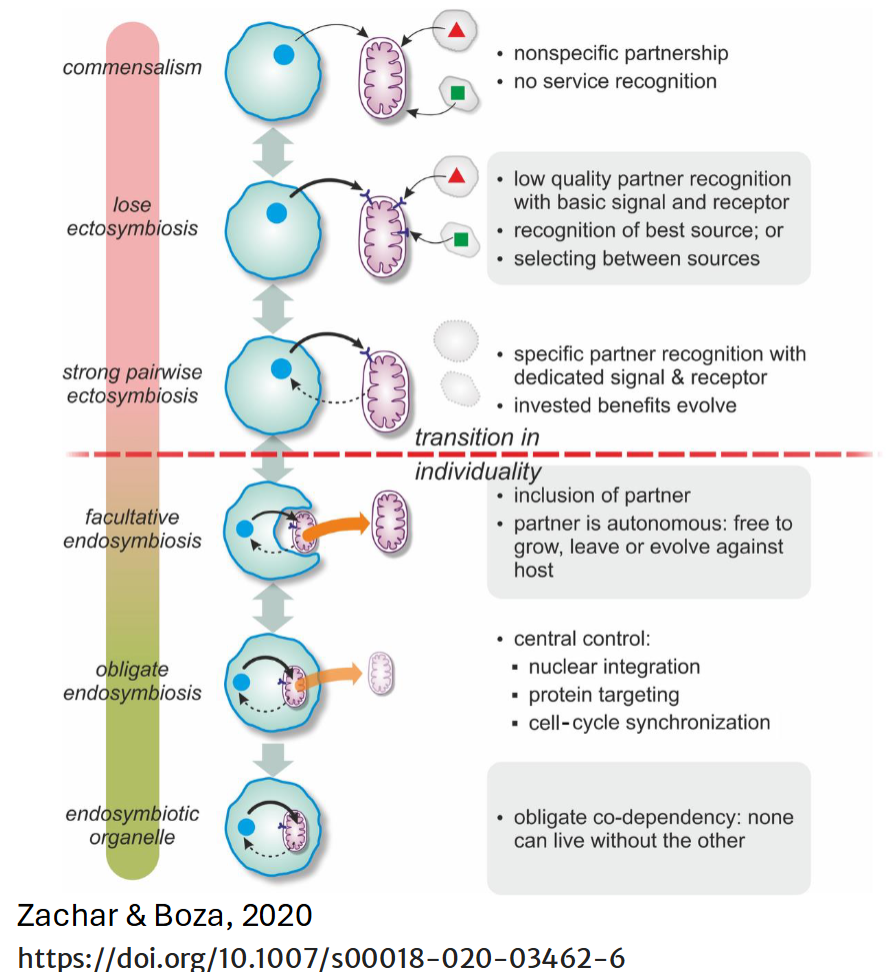
\includegraphics[scale=0.6]{L1_2.png}
\end{center}
\begin{itemize}
    \item Mitochondria used to be separate cells, rather than an organelle.
    \item At some point, one cell engulfed the other, and evolution occured.
\end{itemize}
\subsubsection*{Mitochondria}
\begin{center}
    \includegraphics*[scale=0.6]{L1_3.png}
\end{center}
\subsubsection*{Evolution of Metabolism}
\begin{itemize}
    \item This example alone demonstrates the transformative impact of oxygen in life
    \item \textbf{Biochemistry can be divided into two eras: one before oxygen, and one after}
    \item Modern processes depend on oxygen, while older, more ancient pathways functioned in its absence.
\end{itemize}
\begin{center}
    \includegraphics*[width=\textwidth]{L1_4.png}
\end{center}
\subsubsection*{Proteins}
\begin{center}
    \includegraphics*[width=\textwidth]{L1_5.png}
\end{center}
\begin{itemize}
    \item The above diagram shows proteins, an important part of cells and metabolism.
    \item This class aims to study the metabolic pathways in cells, many of which are catalyzed by proteins (specifically enzymes).
    \item RNA can also be a catalyst.  (RNA is not a protein)
\end{itemize}
\section*{Water}
\begin{center}
    \includegraphics*[width=\textwidth]{L1_6.png}
\end{center}
\begin{itemize}
    \item Water is a dominant metabolite in biochemistry, accounting for 99.4\% by molarity of metabolites within an \textit{E. coli.} bacteria.  Water in an \textit{E. coli} cell is around 40 M.  The sum of the concentrations of all other metabolites is 240 mM.
\end{itemize}
\subsection*{Proteins Exist in Aqueous Environments}
\begin{itemize}
    \item Our first major topic in this class is \textbf{protein synthesis and structure}
    \begin{itemize}
        \item The \textbf{amino acids} of proteins are affected by the \textbf{pH} of aqueous environments (protonation state!)
        \item These amino acids often form different \textbf{intermolecular interactions} amongst themselves and with their environment
        \item The folding of proteins is a \textbf{thermodynamic} problem
    \end{itemize}
\end{itemize}
\subsection*{Importance of Water}
\begin{itemize}
    \item Physical and chemical properties of water influence every biochemical interaction
    \begin{itemize}
        \item The medium for most biochemical reactions
        \item Participates directly in many biochemical reactions
        \item Affects folding (structure) of biomolecules
    \end{itemize}
\end{itemize}

\end{document}
